\thispagestyle{empty}

\begin{center}
{\includegraphics[scale=1.5]{om.eps}}
\end{center}

1 ``satayxjAcnxnAnaMtabarxhamxnU, BAratiVBaratAcAyaRnU, vidAyxrAjanU, jAcnxnayajAcnxmudarxnivxtanU, haMsavijAcnxnoVpadeVshakanU, amaqtarasadhAreyanunx harisutAtx vishavxBaratakekx  sherxVyaH-perxVyasusxgaLanunx niVDutitxruva parxNavahayahaMsaparoVrajanU Ada shirxVmanAnxrAyaNana shuDaraDigaLalilx pArxNagaLanunx bagigxsi parxNAmamADoVNa.

2 ``tirxvikarxmaviSuNxlakiSxmXVnikeVtanavU, shivashakitxsumaMdiravU Ada jAcnxna vijAcnxnamaMdiravoyxVmAMbujadalilx mahaSiRgaLa aMtalaRkapxyXkekx veVdayxnAda savaRvidAyxmUlajoyxVtiyanunx kaMDu BArataBaratarU AnaMdaBaritarU Agi naliyutAtx (nATayxvADutAtx) namamx catuSapxSiTxkalegaLalilx hudugiruva A jAcnxnavijAcnxnamayamahAhayahaMsajoyxVtisasxtXMBada meVliruva mUladiVpadimadx diVpamAlAsahasarxvanunx vishavxvijAcnxnamaMdiradalilx hacicx (hatitxsi) parxjavxlisuvaMte mADoVNa.

3. ``mAhAmasitxSakxveMba jAcnxnavijAcnxnamaMdirada tirxdhAmayutavAda barxhamxmAgaRtatatxvXsoVpAnavishavxraMgAMbujadalilx haMsAsaneyAgi, haMsa gamaneyAgi nAdashabadxbarxhamxrUpiNiyAgi, barxhamxdaMDaniVtiyanunx vivarisuva tirxkAlanADimUtiRsumadxriyAgi, parxmabarxhamxgaqhiNiyAgi, veVdagaBeRyAgi, vishavxceYtanayxsatxnayxdAyiniyAgi, jiVvasumanasavananxraLisuva pArxNashakitxyAgi, barxhamxBAvajoyxVtinARdavijAcnxnavipaMcikeyanunx parxpaMcisi AtamxshirxVyanunx biVruvavaLAgi, namamx maMdirada, haqtamxMdirada mahAmaMgaLAdiVpareVKeyU, vidAyxrANiyU, vishavxshilapxvidhAnajecnxyU Ada mahAnATayxBAratiya padapuMDariVkamahAmadhuvanunx namamx pArxNa madhukaravu pUNaRcaMdirxkeyalilx niranatxravAgi (sadA) pAna mADutitxrali."

\vskip 20pt
\centerline{{\bf OM tatf satf}}
